\chapter{Supernova Remnants: Observation and Theory}
\label{chap:Rems}

\section{\snr{} Identification and Classification}\label{Rems:intro}
When a massive star at the end stage of its evolution explodes as a supernova, it nearly instantaneously injects a massive amount of kinetic energy into the surrounding medium ($\sim 10^{51}$ erg). The supersonically expanding blast-wave, ejected stellar mass, and possible compact stellar remnant comprise an \snr{}. The first two identified \snrs{} (the Crab and Kepler's \snr{}) were initially observed as optical nebulosities found to be associated with historical supernovae (see Figure \ref{fig:Crab}). It was not until the advent of the radio interferometer that a number of these nebulae were discovered and could thus be studied as a population.  In fact, one of the first discrete radio objects to be detected was a remnant in the Cassiopeia constellation now known as Cassiopeia A \citep{Ryle48}.

\begin{figure*}[h!]
	\begin{center}
		%\hspace*{-1.5cm} 
		\begin{tabular}{ll}
			\includegraphics[width=0.5\columnwidth]{Figures/{rosseCrab1}.png} &
			\includegraphics[width=0.5\columnwidth]{Figures/{rosseCrab2}.jpg} \\
		\end{tabular}
	\end{center}
	\caption[Historical Crab nebula drawings]{
		\label{fig:Crab}{Left: First depiction of the Crab nebula by William Parsons, the Third Earl of Rosse,  based on his observations using a 36 inch telescope in 1844. The filamentary structure motivated him to dub it the Crab nebula. Right: Another depiction of the Crab nebula  by William Parson and R. J. Mitchell based on observations with a 72 inch telescope in 1884. From J. Bevis, Uranographia Britannica, 1750}
	}
\end{figure*}
One of the primary distinguishing features of the radio emission from \snrs{} was their distinctly non-thermal spectra (a \pl{} with flux  ${\rm S \propto \nu^\alpha}$, where $\nu$ is frequency). The clearly non-thermal emission was first proposed to arise from \sync{} radiation (and hence emitted by a population of relativistic electrons) by \cite{Kiepenheuer50} and \cite{Alfven50}, and then by \cite{Shklovskii53} who correctly associated the remnants with supernovae in the Galaxy. To this day, \snrs{} are still primarily identified through radio observations (although a number have been first detected in X-ray as well). A catalog of 294 radio-identified Galactic \snrs{} is maintained at \url{http://www.mrao.cam.ac.uk/surveys/snrs/} by \cite{Green14} (referred to as Green's catalog) and a complementary high-energy catalog, summarizing \snr{}  X-ray to \gam{} properties, is upkept by \cite{Ferrand12} at \url{http://www.physics.umanitoba.ca/snr/SNRcat}

While the nonthermal, radio \sync{} spectra of  \snrs{} are used to identify remnants, their morphology is used to classify them. The classifications, based on radio and X-ray observations are:
\begin{itemize}
	\item \textbf{ Shell-type} \snrs{} are characterized by a radio (and sometimes X-ray) limb-brightened shell or ring. The perimeter or the (possibly incomplete) shell corresponds to the expanding forward shock from the blast-wave and is composed of the ejecta from the initial explosion as well as mass from the surrounding medium swept-up by the blast-wave. They are typically associated with less-evolved, or dynamically young \snrs{} (see the following Chapter for details on \snr{} evolution). In \cite{Green14} 79\% of the radio \snrs{} are classified as shell type. 
	
	\item \textbf{Filled-center} \snrs{} or \textbf{plerions} are \snrs{} that show no clear shell structure but  rather are centrally bright at radio, and sometimes X-ray, energies. The central \sync{} emission arises if the  compact stellar remnant is a pulsar which can drive a \pwn{} \cite{Gaensler06}. The \pwn{} is generated by the rotational power of the spinning pulsar transferring its energy to a relativistic, magnetized wind of electrons and positrons that emit \sync{} radiation throughout the nebula. While the energy source of the shell-type \snr{} is deposited in the singular supernova event, the spin-down power of the pulsar is injected into the plerionic system over a much longer time span. 5\% of radio \snrs{} are center-filled \citep{Green14}.
	\item \textbf{Composite} remnants are simply \snrs{} that display both a  distinct shell-like structure as well as a center-filled, non-thermal \sync{} nebula.. \cite{Green14} classifies 12\% of \snrs{} as being composite.
	
	\item \textbf{Mixed morphology} \snrs{} are ones that exhibit a non-thermal radio shell-like structure as well as centrally located thermal X-ray emission \citep{Rho98}. This is in contrast to the composite system which displays a non-thermal emission nebula generated by a rotating neutron star. Some authors, including \cite{Green14} use mixed-morphology interchangeably with composite. The thermal X-ray emission is produced by swept-up and shock-heated  material. These \snrs{} are often associated with more-evolved (or middle-aged) remnants that are interacting with surrounding, dense molecular material (as evidenced by shocked molecular lines and sometimes 1720 MHz OH masers). As t
	\jamie{add kewl pic of each of the types shell:casA, tycho, kep, young! plerion: crab 3C58. comp: Vela?, mixed:IC443?}
\end{itemize}

The remaining few percent of \snrs{} not classified as one of the above are remnants that show a more complicated morphology, yet are still believed to be \snrs{}. In fact, with more sensitive, higher resolution telescopes, many shell-type \snrs{} only exhibit partially complete circular structures, and may show signs of blow-out (when part of the shell appears to expand faster in one direction than another) or elongated morphologies, all signs of not-purely spherical evolution of the blast-wave (which itself might not be spherically symmetric) in an inhomogeneous \ism{}.

\section{\label{Rems:evo}\snr{} Dynamics and  Evolution}
The formation of an \snr{} begins as the supersonically traveling ejecta expands out and collides with the \ism{}  forming a blast-wave. The standard model for the evolution of an \snr{} (first proposed by \cite{Woltjer72}) is divided into four phases. 

\begin{enumerate}
	\item \textbf{ Free-Expansion Phase:} In this phase, (sometimes referred to as the ejecta-dominated phase), the forward shock of the blast-wave expands out into the \ism{} sweeping up mass as it expands. The ejecta mass is of the order of a few to 10's of \msun{}, while the shock speed is typically ${\rm \sim 10^3-10^4~ km~s^{-1}}$ for type Ia and core-collapse events respectively \cite{Reynolds08}. The velocity of the shock remains essentially constant in this phase until the mass of the swept-up material, equals that of the ejecta mass.
	At this point the swept-up mass starts to dynamically affect the expansion of the remnant, marking the end of the free-expansion phase.
	
	\item \textbf{\sedt{} Phase:} The \sedt{} phase (also referred to as the adiabatic expansion phase) begins when the swept-up mass ${\rm M_{su}}$, is equivalent to the ejecta mass, ${\rm M_{ej}}$. The radius of the \snr{} at the onset of the \sedt{} phase is given by:
	 
	\begin{equation}
	R_{ST_0} = (3M_{ej}/4\pi \mu \rho_0)^{1/3} = 1.9(M_{ej}/n_0)^{1/3} pc,
	\end{equation}
	for ${\rm \rho_0 = n_0m_H}$, the mass density of the swept up matter, where 
	${\rm n_0}$ is the pre-shock particle density of the medium the \snr{} is expanding into (in units of ${\rm cm^{-3}}$), $\mu\approx1.4$ is the \ism{}'s mean atomic weight and ${\rm M_{ej}}$ is in units of \msun{}. The \sedt{} phase is dominated by the thermal pressure of the shock-heated gas which is adiabatically expanding (conserving energy), yet the gas is still hot enough that radiative losses are relatively inefficient. \cite{1959sdmm.book.....S} and \cite{Taylor50} developed a self-similar, analytic model for the evolution of the shock at this phase for an explosion that instantaneously injects energy at a point into a uniform density medium with no energy loss. The \sedt{} solution for the radius of a shock that evolves with time, t, for an explosion energy, E, is:
	\begin{equation}
	R_{ST} = \bigg{(}\zeta \frac{Et^2}{\rho_0} \bigg{)}^{{1/5}} = 0.314(E_{51}/n_0)^{1/5}t_{y}^{2/5} pc,
	\end{equation}
	with the constant, $\zeta = 2.026$ corresponding to a monatomic, non-relativistic  gas ($\gamma = 5/3$), E$_{51}$ the energy of the explosion in units of $10^{51}$ erg, and t given in years. This phase typically lasts for a few $10^4$ yr, when the radius of the \snr{} is 10's of pc. The \sedt{} phase ends when the temperature has decreased enough ($\approx 10^6 K$), through expansion and adiabatic cooling, that recombination can occur and atoms can cool radiatively.
	
	\item \textbf{Radiative Phase:} In the radiative phase, also known as the snowplow phase, the increased cooling causes the \snr{} shell to expand slower. Interior to the shock though, hot gas has not had time to cool and continues expanding adiabatically, exerting a pressure on the cooler, outer shell. The pressure of the hot interior pushes on the dense shell,  ``snowplowing'' ambient mass from the \ism{}, which will coast out, conserving momentum as the interior cools. 
	\item \textbf{Dispersion Phase:} Finally, the \snr{} diffuses and merges into the \ism{} with the temperature and shock velocity decreasing and becoming comparable to that of the ambient \ism{}.
\end{enumerate}

While this general scheme for the evolution of an \snr{} in the \ism{} is sufficient for explaining general observational features of \snrs{}, more intricate models are required to explain details of individual \snrs{}. Various authors have since expanded on the dynamical evolution of \snrs{} by including information regarding the initial velocity/density structure of the ejecta, inhomogeneities of the material the \snr{} is expanding into, energy loss through escaping \crs{}, and the effects of magnetic fields on expansion \citep[and references in \cite{Vink12} which reviews various analytic \snr{ expansion models}]{Chevalier74,Chevalier82,Truelove99}.
  
\section{\label{Rems:CR}The SNR Cosmic Ray connection}

\cite{Baade34}
\cite{Ginzburg64}
\cite{Hayakawa69}

driver of Galatic blah
Give the whole, if 10\% of energy of SN explosion goes into particle acceleration, we can explain cosmic rays

Particle acceleration and DSA

radio index to particle index

power law form for aprticle spectra (this is from dsa)
This leads to gamma-ray section




\section{\label{Rems:latGam}Supernova Remnants at \gam~Energies}

By the end of the its science run, \egret{} had detected 271 sources above 100\mev{}, within a minimum detection significance of 4$\sigma$, 170 of which had no clear multiwavelength counterpart, with 81 of those unidentified lying within \blat of the Galactic plane \citep{Hartman99}. The main hindrances to source identification were the numerous potential source counterparts (the \egret{} \psf{} was energy dependent, with a 68\% containment radius of ${\rm \sim 6 ^\circ}$ at 100\mev{} and smaller for higher energies) and the large \egret{} error boxes. In addition to this, the primary method for identifying a \gam{} source as an \snr{} is through a compatible angular extent with  observations at some other wavelength, thus the ability to resolve emission from an \snr{} is vital to understanding the mechanisms therein giving rise to \gam{}s. Figure \ref{fig:3EGSky} shows an \egret{} all-sky map at ${\rm E > 100 \mev}$ where the preponderance of unidentified sources and locations thereof are made clear.

\begin{figure}[h!]%[t] 
	\centering
	\makebox[\linewidth]{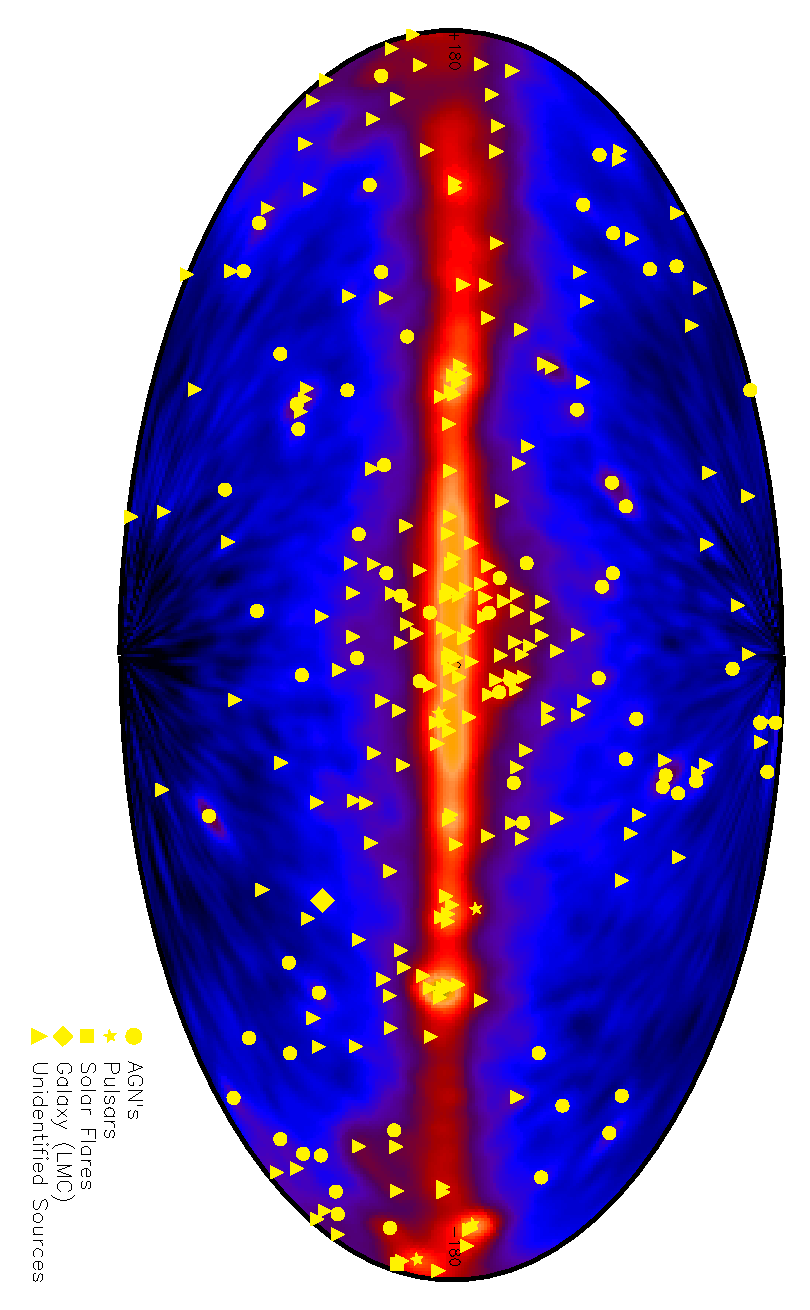
\includegraphics[width=0.8\columnwidth,angle=90]{Figures/3rd_egret_cat.eps} }
	\caption[Third EGRET catalog all-sky map.]{Third EGRET catalog all-sky map. Unidentified sources represented by triangles. Image courtesy of \url{https://heasarc.gsfc.nasa.gov/docs/cgro/images/epo/gallery/skymaps/}}
	\label{fig:3EGSky} 
\end{figure}

In spite of the difficulties in \egret{} source association, many studies have attempted correlating the unidentified \egret{} sources with various Galactic populations. In particular, several authors found strong evidence for statistical correlation between \glspl{snr} and some of the low-latitude unidentified sources \citep{Sturner95, Esposito96, Romero99}. In a review of the state of potential \snr{} /  \egret{} associations, \cite{Torres03} showed that there were 19 unidentified \egret{} sources that had an \snr~fall within its 95\% error box. Performing Monte Carlo simulations of the population of  \egret~sources, they determined that the chance probability for the 19 sources to be coincident with an \snr~was $1.05 \times 10^{-5}$, implying a probability of 0.99998 that at least one of the associations is real. Despite the statistical correlation of \egret~sources with \glspl{snr}, there were no definitive associations of an \snr~with any \egret~sources.

As the successor to \egret{}, the \lat{} was designed to improve upon its predecessor in a multitude of areas relevant to detecting \snrs{} \citep{atwood09,lat_perf}. The \lat{} has a much improved angular resolution (68\% single-photon containment radius $\sim 0.4^{\circ}$ at 1\gev{} for photons with the best quality direction reconstruction, PSF3 event type, compared to $\sim 1.7^{\circ}$ for \egret{} at the same energy), necessary to resolve \snrs{} as extended objects. The \lat{} also benefits from a superior sensitivity due to a combination of the improved \psf, larger peak effective area ($ {\rm > 9000~cm^2}$ vs. ${\rm \sim 1500~cm^2}$), wider \fov{} (2.4 sr, which is nearly 5 times that of \egret{}), and deeper, more-uniform sky exposure (afforded by the \lat's scanning observations as opposed to \egret's pointing operation). 

This bump in sensitivity results in the \lat{} detecting considerably more sources than \egret. Remarkably, within its first three months of commission, the \lat{} detected 205 sources above {\rm 10$\sigma$ significance \citep{lat_3m}, and by 11 months, 1451 sources above 4$\sigma$ \citep{1FGL}, compared to  the aforementioned 271 over the entire \egret{} mission. In fact, over its lifetime, \egret{} detected a total of about ${\rm 1.5~x~10^6}$ cosmic photons \citep{Thomson93}, while as of March 2016, the \lat{} has detected ${\rm \sim 863~x~10^6}$ \jamie{change this number in June} source class photons. The \lat's point-source sensitivity peaks between 1 and 10\gev{}, depending on location on the sky. With its increased sensitivity and higher energy range (up to $\sim$ 2\tev{} with the recent Pass 8 event reconstruction improvements, which is nearly an order of magnitude higher than \egret{}), the \lat{} is uniquely situated to study the \gam{} morphology and spectra of \snrs{}.
	
Both energetic lepton interactions (\ie \ic{} radiation of relativistic electrons interacting with ambient photon fields, and nonthermal \brems{}) and hadronic processes ($\pi_0$ decay \gam{}s from \cray{} protons encountering surrounding nuclei) produce spectra observable at \gam{} energies (see Chapter \ref{chap:gamAstr} for details). While the \ic{} generating electron population is also observable through emission of radio \sync{} photons, the proton-proton interaction solely emits \gam{}s. Despite being the prime energy range to observe the effects of cosmic particle acceleration, complexities at the lower \lat{} energy range stymie \snr{} morphology studies.
	
The \lat{} detects a strong, soft band of diffuse emission in the Galactic plane due to the interactions of  \crs{} with interstellar material. This bright diffuse radiation combined with the multiple potential emission scenarios, broadening \psf{} at decreasing energy, and a high source density in the plane can make it difficult to spatially disentangle sources observed by the \lat{}. To circumvent these 
difficulties, the majority of the analyses undertaken in this thesis are focused on the ${\rm E \geq 1\gev}$ energy range. This energy band is ideal for probing the properties of the accelerated particle populations present in the \snr{} environment. Studies of  \snrs{}  above 1\gev{} benefit from finer \lat{} \psf{}, striking a balance between minimizing the diffuse contribution, maximizing photon sensitivity, and retaining good photon statistics. Furthermore, evolved \snrs{}  exhibit a spectral break between 1-10\gev{} \citep{Hewitt15}. Explanations for the break range from Alfv\' en wave evanescence generated by collisions of partially ionized material in \mcs{} overtaken by \snr{}  shocks \citep{Malkov11}, reflected shocks in clouds \cite{Inoue10c}, and energy-dependent diffusion from shocks \cite{Ohira11}. Studying \snrs{} in this energy range hones our capability to tackle several goals set out by the \Fermi{} team when the mission was conceived.
\jamie{in the next chapter we describe the population of GeV. something about what was detected before the snr cat?}


Go into current state of gamma obs, LAT, TeV
what they probe etc
\jamie{something about TeV observations. Predominantly young or parts of interacting rems (like the signs of escape) 12 shell type, 1 composite 7 SNR/MC. see https://arxiv.org/pdf/1508.05190v1.pdf or https://arxiv.org/pdf/1510.01373v1.pdf}


\snr{I need to end with something about how/why awesome \Fermi{} has and will continue to be in searching for SNRs?mmaybe}
\section{Summary}\label{Rems:summ} In this section we summarized the end phase of stellar evolution (just enough to motivate SNRs) and descried the environs surrounding the supernova; development and phases of \glspl{snr} (and \glspl{pwn}?).  In particular we detailed the nonthermal emission mechanisms that produce \g-ray radiation, detection of young vs middle-aged( evolved, interacting with surroundings/dense medium),TeV detects younger typically, the troubles of detecting extension from them(?) something about different emission zones? Troubles disentangling hadronic from leptonic at \g-rays. \g-ray spectral and morphological features. Trends across the population wrt spectral shape/breaks, higher luminosity for interacting rems. Cosmic rays, using gamma-rays to probe CR population. So much of \g-ray astro is really about studying CRs, how much to say about them? 

\section{Scratch}
This chapter needs a different title. It's more focused on the specific sources being studied in this thesis. Galactic extended sources, SNRs, PWNe, but as in the SNRcat, not just extended SNRs, point-like SNRs as well.

Less focus on PWNe. Only give as much as I feel I need to support mentioning them a bit for 2FHL?

The focus of this section is supernova remnants in a gamma-ray context. Theory of evolution, what the gamma-ray emission is like, what we can learn from them individually.  This leads to the 1st SNR cat section for what we can do with them ensemble

NOt sure I really need any PWN stuff yet

in 2FHL we detect some pwn. If including above 10gev work, they'll be there too. Much of the thesis is really about extended gamma-ray sources, but not sure how that fits into the title and chapters yet

Do I need to get into composite SNRs (composite means SNR + PWN ) Maybe relevant for G150? Some things about interaction of reverse shock with PWN and crushing/reverberations of the PWN?

\cite{Montmerle79}